\chapter{Background}

This chapter aims to explain the basic concepts that are the most important to the work in this thesis.



% -------------------------------------------------------
% -------------------------------------------------------
% ---------------------- Graphs -------------------------
% -------------------------------------------------------
% -------------------------------------------------------
\section{Graphs}
\subsection{Nodes and Edges}
\subsection{Directed Acyclic Graphs}




% -------------------------------------------------------
% -------------------------------------------------------
% ----------------- Machine Learning --------------------
% -------------------------------------------------------
% -------------------------------------------------------
\section{Machine Learning}

The following sections will define the term 'Machine Learning'. 
It will describe some various ways that machine learning can be applied.



\subsection{What is machine learning?}

As a term, 'Machine Learning' is a subcategory if the umbrella term 'Artificial Intelligence'.
It is proposed as an alternative to traditional algorithms. 
Machine Learning takes a set of input (training) data, and attempts to reason about some quality of the input, 
without the author of the program explicitly telling the program what quality of the input data we are interested in reasoning about.
Instead, the author provides the Machine Learning model with their optimal target for the given input,
and the model must attempt to generalize over, and design its own algorithm to fit the target.

This approach has become useful in problems where discovering the target based on the model input becomes computationally intractible,
or when the target cannot be determined as a direct consequence of the input. 
An example of such a problem is sentiment analysis of text input. 
Given the sentence 'The nice boy made fun of the kind girl', 
it is difficult to design rules which can capture the sentiment of the sentence.
On one hand, the words 'nice', 'fun', and 'kind' indicate this sentence may have a positive sentiment.
In reality, our ability to reason tells us that this is not the case, and the sentence is of a negative nature.

\textbf{Noen ord her om Classification vs Regression. Hva er forskjellen - hva er greien?}


\textbf{Machine Learning is deeply rooted in Bayesian Statistics. (Noen gode setninger om bayes. Gjerne bayes teorem? Ikke mer enn et avsnitt. Dette er en AI-oppgave, ikke en statistikk-oppgave.)}


\subsection{Linear Regression}
\label{subsection:linreg}

As a first study in the implementation of machine learning, we look at linear regression.
To explan linear regression, we view an example in a two dimensional, euclidean space.
We are given a set of input data values $ X $ . Each input value $ x_i \in X $ has a corresponding output value $ y_i \in Y $.
We can plot each input value, and its corresponding output value as coordinates.


To describe a function that best maps the given inputs with their related outputs, 
we introduce two variables $ w_0 $ and $ b_0 $. We define a function to map our input values to their corresponding output.

\[
        f(x) = w_0x + b \tag{2.1} \label{linreg}
\]

We also introduce some measure of how well our function $ \eqref{linreg} $
maps our input to our output. As we tune our function variables $ w_0 $ and $ b_0 $ to better map the input to its corresponding output,
the measure will decrease. There exists values for our variables $ w_0 $ and $ b_0 $  such that the measure defined in $ \ref{func:mse} $ reaches its lowest possible value.
In this state, the function optimally maps the input data to with its corresponding output, given our function.

\[
    \mathcal{L} = \frac{1}{|X|}\sum_{i = 0}^{|X|} \big(y_i - f(x_i)\big)^2 \tag{2.2} \label{func:mse}
\]

Of course, the function defined in $ \eqref{linreg} $ is arbitrary. 
We can add or remove existing or additional function variables as we wish,
if we see that changing the function structure improves at mapping the input to the output.
This example has applied linear regression to single-dimensional inputs and single-dimensional outputs,
but the same method can be applied to inputs and outputs of higher dimensions.
The method can also be applied when the inputs and outputs are of different dimensions, by applying linear transformations.
A general formula for linear regression can therefore be 



\[
    X \in \mathbb{R}^m, \{Y, b\} \in \mathbb{R}^n, W \in \mathbb{R}^{m x n}
\]
\[
    f(X) = WX + b \tag{2.3} \label{func:linearLayer}
\]
 

\begin{figure}
    \centering
    \subfloat[\centering Input x values plotted against their corresponding y values]{{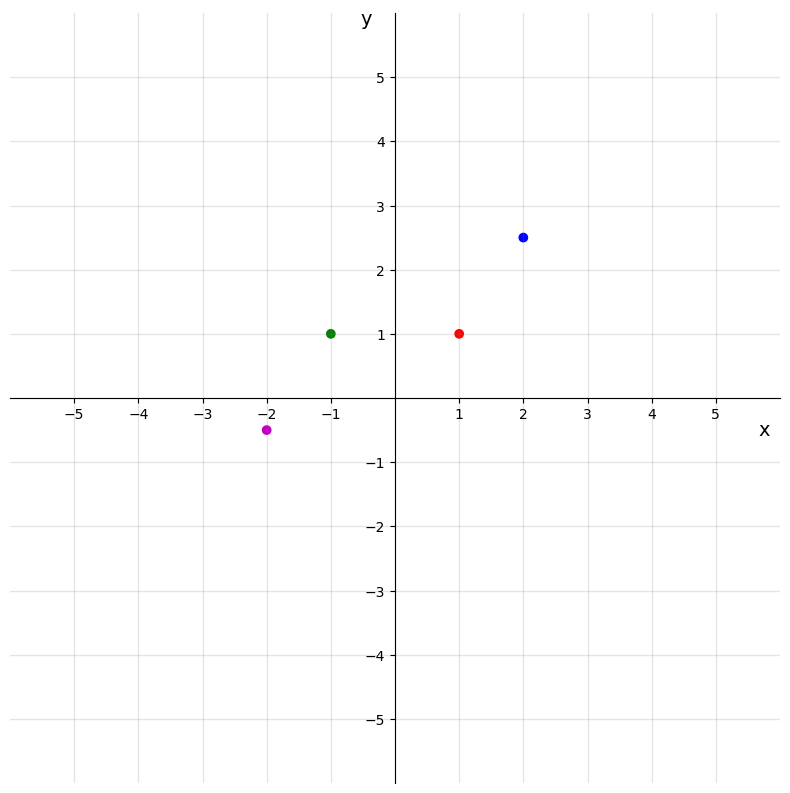
\includegraphics[width=7cm]{figures/background/linreg_input_illustrated.png} }}%
    \qquad
    \subfloat[\centering Function $ \eqref{func:mse} $ applied to function $ \eqref{linreg} $ with optimized function variables $ w_0 $ and $ b_0 $]{{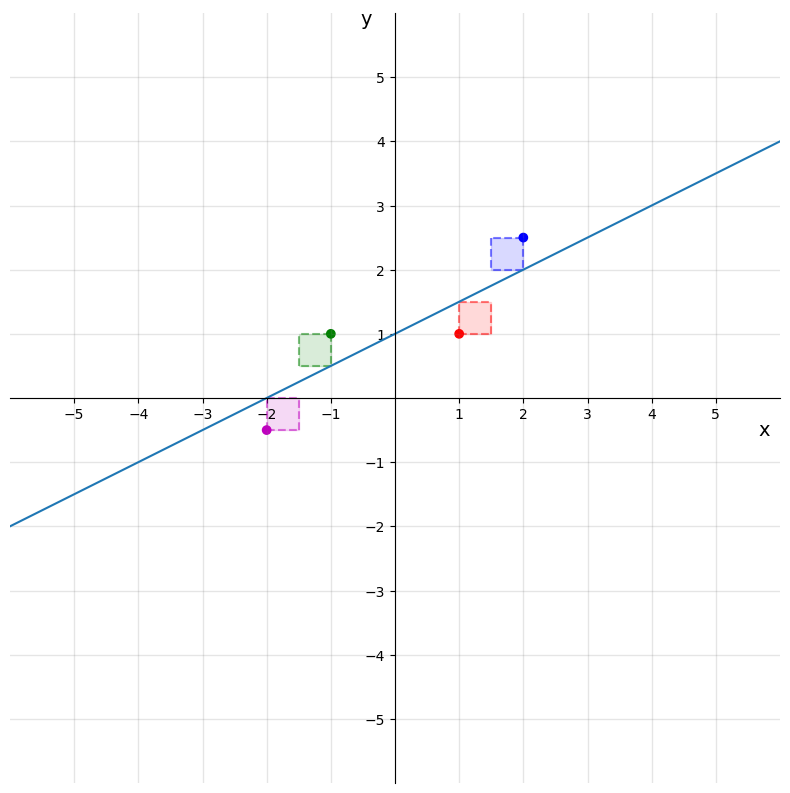
\includegraphics[width=7cm]{figures/background/MSE_illustrated.png}}}
    \caption{Linear regression illustrated}%
    \label{fig:linearRegression}%
\end{figure}



\subsection{Loss}
\label{section:loss}

In the previous section, a measure of how 'wrong' a mapping of input points to their corresponding output points was defined.
In the litterature, this measure is referred to as the loss function. 
The loss function defined in $ \eqref{func:mse} $ is named 'Mean Squared Error Loss', 
due to the fact that it is defined by the mean of the squared difference between our function's predictions and the true values.
The 'Mean Squared Error Loss' operator is referred to as 'MSE' for the rest of this thesis.

It is possible to define different loss functions. A loss function must be nonnegative for all input values.
Different loss functions will interpret the performance of a functions mapping of the given input data to its corresponding output in different ways.
The difference in ... can be illustrated by observing the result of applying the loss function defined in $ \eqref{func:mae} $, typically referred to as 'Mean Absolute Error Loss', shortened to 'MAE' in this thesis, as opposed using MSE.

\[ 
    \mathcal{L} = \frac{1}{|X|}\sum_{i = 0}^{|X|} \sqrt{\big(y_i - f(x_i)\big)^2} \tag{2.4} \label{func:mae} 
\]

While MSE loss sums over the squares of errors, MAE sums over the absolute errors.
Using MAE, each prediction's error term will grow linearly, given the true output value.
Using MSE, however, each prediction's error term will grow exponentially, given the true output value.
As a consequence, 'MAE' will place equal weight emphasis on each prediction's error.
MSE will place more emphasis on predictions that are further from the true output values.
Different loss functions can therefore be applied to different problems to find different solutions. 
Figure $ \eqref{fig:lossFunctions} $ illustrates an example of different loss functions being applied to the same prediction function.
The optimal function parameters were found using the MAE operator. When the MSE operator is applied to the same function parameters,
the MSE operator does not produce its lowest possible value.

\begin{figure}
    \centering
    \subfloat[\centering Loss function $ \eqref{func:mae} $ applied to function $ \eqref{linreg} $ with optimized function variables $ w_0 $ and $ b_0 $ ]{{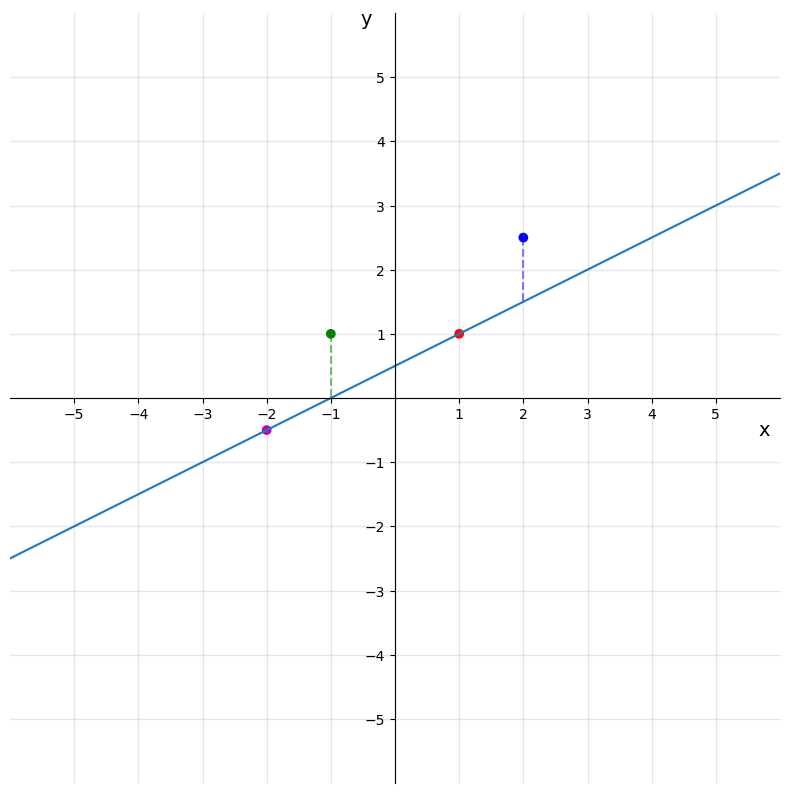
\includegraphics[width=7cm]{figures/background/loss/mae_optimal.png}}}
    \qquad
    \subfloat[\centering Loss function $ \eqref{func:mse} $ applied to function $ \eqref{linreg} $ with function variables $ w_0 $ and $ b_0 $ optimised using  loss function $ \eqref{func:mae} $ ]{{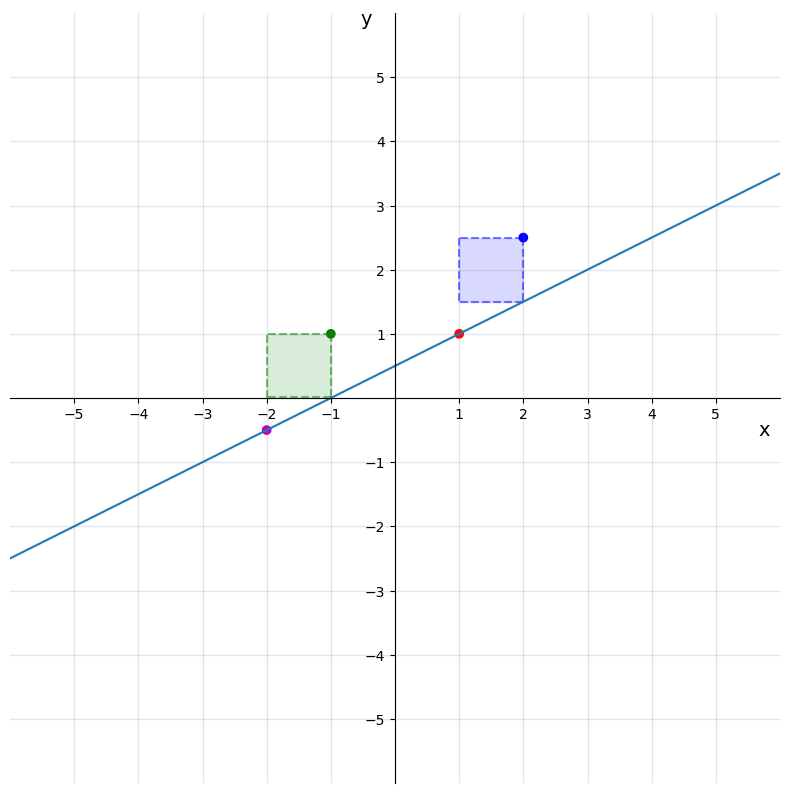
\includegraphics[width=7cm]{figures/background/loss/mse_not_optimal.png} }}%

    \caption{Different loss functions applied to the same prediction function}%
    \label{fig:lossFunctions}%
\end{figure}

The loss functions presented so far in this section have all been focused on the regression task in machine learning applications.
For prediction tasks, a better suited loss function should be used. A common loss function for this kind of task
is the cross entropy loss function, defined in $ \eqref{func:crossentropy} $.

\[
    \mathcal{L} = - \sum_{i = 0}^{|X|}p(y_i) log\big(f(x_i)\big)
    \tag{2.5} \label{func:crossentropy}
\]



\subsection{Underfitting and overfitting}

\subsection{Supervised and unsupervised learning}




\section{Neural Networks}




This section aims to explain the foundational concepts of what is today referred to as Neural Networks.
In section \ref{subsection:linreg}, the idea of Linear Regression was introduced.
As the foundational concepts of neural networks are introduced, it is useful to keep the idea behind Linear Regression in mind.

The explanation of Neural Networks is broken down into four parts. 
First, two curical concepts are introduced, namely 'Linear layers' and 'activation functions'. 
Then, this thesis assesses what is referred to as the 'forward pass', as this is the simplest to explain.
Finally, the 'optimization step' is assessed.




\subsection{Activation functions}
\label{subsection:activationFunctions}


Activation functions are a set of non-linear functions that are utilised in neural networks to ensure non-linearity between the network layers.
An activation function may take many forms, as any non-linear mapping of input values, defined on all real numbers, will function as an activation function.



\subsubsection{Sigmoid}

The sigmoid function maps any given input value to a value between 0 and 1. 




\[
    Sigmoid(x) =  \frac{1}{1 + e^{-x}}
    \tag{2.6} \label{func:sigmoid}
\]

\subsubsection{ReLU}

The (Re)ctified (L)inear (U)nit maps any given input value to a value greater than 0, with no upper limit.

\[
    ReLU(x) =
    \begin{cases}
        0,& \text{if } x < 0\\
        x,& \text{if } x\ge 0
    \end{cases}
    \tag{2.7} \label{func:relu}
\]

\textcolor{red}{\textbf{Vis is den deriverte her og snakk om den også?}}





\subsection{Linear layers}
\label{subsection:linearLayers}

To introduce linear layers, recall the multi-dimensional regression formula defined in equation \ref{func:linearLayer}.
In the litterature, linear layers may be referred to using various titles. 
Among the most common names for this kind of function are 'Dense layers', 'Fully connected layers' or 'Multi layer perceptrons'.
\textcolor{red}{\textbf{(Finn eksempler og legg inn referanse)}}
The aforementioned titles all refer to an implementation of the formula \ref{func:linearLayer}. 
For the purposes of this theses, the term 'Linear layers' will be used to denote this concept.

The linear layer is the quintessential building block of neural networks. 
Though more advanced layers for use in Neural Networks have been developed since linear layers were introduced, 
linear layers are still a very common building block in modern network architectures. 

Linear layers differ from multidimensional linear regression in the fact that the parameters of the linear layer are no 
longer solved for the optimal solution of the input data.
Instead, both the linear layer's weight- and bias terms, constituting the linear layer's parameters, are initialised randomly\textbf{\textcolor{red}{(obs, ikke helt random. Ofte trekt fra normaldistribusjon? Sjekk hva torch geometric gjør.)}}, 
and their optimal values are approached using some algorithm. This algorithm will be discussed further in section \ref{subsection:optimizationStep}.




\subsection{Neural Network Structure}

Using the combined elements defined in sections \ref{subsection:linearLayers} and \ref{subsection:activationFunctions}, 
a sample Neural Network can be constructed. Furthermore, this Neural Netowrk can be used as a tool to explore the functionality of Neural Networks

Assume a learning task where a ($ n_0 \times m_0 $)-dimensional matrix is given as input, and a ($ n_t \times m_t $)-dimensional output is desired. 
For a classification task, the output is often a ($ num\_classes \times 1 $)-matrix. 
For a regression task, the output may be a  ($ 1 \times 1 $)-matrix, a reconstruction of the input data, eg. a ($ n_0 \times m_0 $)-dimensional matrix, 
or any other shape that fits the task at hand.
A neural network can be constructed to fit this description.

A neural network consists of a series of linear layers performing a linear transformation of the output of the previous layer.
The shape of the each linear layer's weight and bias matrix is determined by the previous layer's output shape, 
as well as the desired input for the next layer. Except for the last layer, each linear layer is followed by an activation function.


\subsection{Example Neural Network}
\label{subsection:sample_network}

To illustrate the inner workings of neural networks, an example neural network is provided. 
The neural network accepts as input a $ 4 x 2 $ value matrix, and outputs a matrix with the same proportions.
Assume a two layer neural network in which the input is projected into the lower, $ 2 x 2 $ dimensional space, is desired.
The ReLU activation function is applied as a non-linearity.


\subsubsection{Input}
\[
X_0 = 
\begin{bmatrix}
    x^{0,\space 0}_0 & x^{0,\space 1}_0 \\
    x^{1,\space 0}_0 & x^{1,\space 1}_0 \\
    x^{2,\space 0}_0 & x^{2,\space 1}_0 \\
    x^{3,\space 0}_0 & x^{3,\space 1}_0
\end{bmatrix}
\]


\subsubsection{First layer}
In the first layer, initialise a weight matrix such that the linear transformation of out input and the weight matrix yields a matrix with desired dimensions.
In this case, the weight matrix is a $ 2 x 4 $-dimensional matrix, such that the matrix product of the weight matrix and the input matrix is a $ 2 x 2 $-dimensional matrix.
\[
W_0 =
\begin{bmatrix}
    w^{0,\space 0}_0 & w^{0,\space 1}_0 & w^{0,\space 2}_0 & w^{0,\space 2}_0 \\
    w^{1,\space 0}_0 & w^{1,\space 1}_0 & w^{1,\space 2}_0 & w^{1,\space 2}_0
\end{bmatrix}
\]

In addition to the weight matrix, a bias term matrix is initialised. This matrix is added to the matrix product of the weight matrix and the input matrix.
\[
B_0 = 
\begin{bmatrix}
    b^{0,\space 0}_1 & b^{0,\space 1}_1 \\
    b^{1,\space 0}_1 & b^{1,\space 1}_1
\end{bmatrix}
\]

Matrices $ W_0 $ and $ B_0 $ contain the trainable parameters for this linear layer.
This linear layer's output can be calculated by performing the linear transformation as described, adding the bias term, and performing the ReLU activation function on the result.

\[
Y_1 = ReLU(W_0 X_0 + B_0) = 
\begin{bmatrix}
    y^{0,\space 0}_1 & y^{0,\space 1}_1 \\
    y^{1,\space 0}_1 & y^{1,\space 1}_1 \\
\end{bmatrix}
\]

\subsubsection{Second layer}
Similarly, for the second layer, initialise a weight matrix such that the linear transformation of the weight matrix and the output of the previous linear layer yields an output which matches our desired properties.
In this case, such a weight matrix is $ 4 x 2 $-dimensional.
\[
W_1 = 
\begin{bmatrix}
    w_1^{0,\space 0} & w_1^{0,\space 1} \\
    w_1^{1,\space 0} & w_1^{1,\space 1} \\
    w_1^{2,\space 0} & w_1^{2,\space 1} \\
    w_1^{3,\space 0} & w_1^{3,\space 1}
\end{bmatrix}
\]

Again, a bias term matrix is intialised with the same dimensions as the linear transformation of the weight matrix and the output of the previous layer.
\[
B_1 = 
\begin{bmatrix}
    b_1^{0,\space 0} & b_1^{0,\space 1} \\
    b_1^{1,\space 0} & b_1^{1,\space 1} \\
    b_1^{2,\space 0} & b_1^{2,\space 1} \\
    b_1^{3,\space 0} & b_1^{3,\space 1}
\end{bmatrix}
\]


Calculate the network's output multiplying the weight matrix with the output of the previous layer, and add the bias term.
\[
\hat{Y} = W_1 Y_1 + B_1 =
\begin{bmatrix}
    \hat{y}^{0,\space 0} & \hat{y}^{0,\space 1} \\
    \hat{y}^{1,\space 0} & \hat{y}^{1,\space 1} \\
    \hat{y}^{2,\space 0} & \hat{y}^{2,\space 1} \\
    \hat{y}^{3,\space 0} & \hat{y}^{3,\space 1}
\end{bmatrix}
\]

Note that no activation function is applied to the output of the last layer. 
Applying the ReLU function in this scenario would cause the network's projection space to be limited to the positive real numbers.
Somewhat similarly, applying the sigmoid function would limit the network's projection space to real numbers between 0 and 1. 
This is not to say that the output of the linear transformation and the bias term cannot be altered to fit the given objective.
Such may be the case in a scenario where the task is to predict a probability distribution. For the purposes of this example, no such alteration is needed.

The propagation of the input variable through the network can be illustrated as in figure \ref{fig:sample_network}.


\begin{figure}
    \centering
    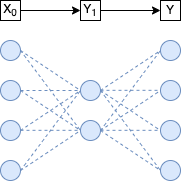
\includegraphics{figures/background/sample_network.png}
    \caption{The network from section \ref{subsection:sample_network} illustrated}%
    \label{fig:sample_network}%
\end{figure}




\subsection{Forward Pass}

During the forward pass, input data is passed through all the layers and activation functions constituting our Neural Network. 
Matrix multplications followed by activation functions are applied to the input data, until some output is achieved, following the last layer.

As defined in section \ref{section:loss}, a loss function is then applied to the output of the linear layer, yielding a measure of the 'closeness' of the neural network's approximated output, and the desired output.
During training, the initial forward passes of any neural network with a given architecture will return a random output in dimensions specified by the architecture.



\subsection{Optimization Step}
\label{subsection:optimizationStep}

The process of optimizing a neural network model is commonly referred to as the 'optimization step'.
The goal of the optimization step is to optimize the model parameters such that for any given input,
the model provides the desired output. Many algorithms have been created to perform this task.
One common such algorithm is the Gradient Descent algorithm. In this thesis, 
the Gradient Descent algorithm will be used to discuss the implementation of the optimization step.
Furthermore, successors of Gradient Descent will be discussed.


\subsubsection{Gradient Descent}

\begin{figure}
    \centering
    \subfloat[\centering A model parameter's current value as well as it's derivative, headed towards the global minimum.]{{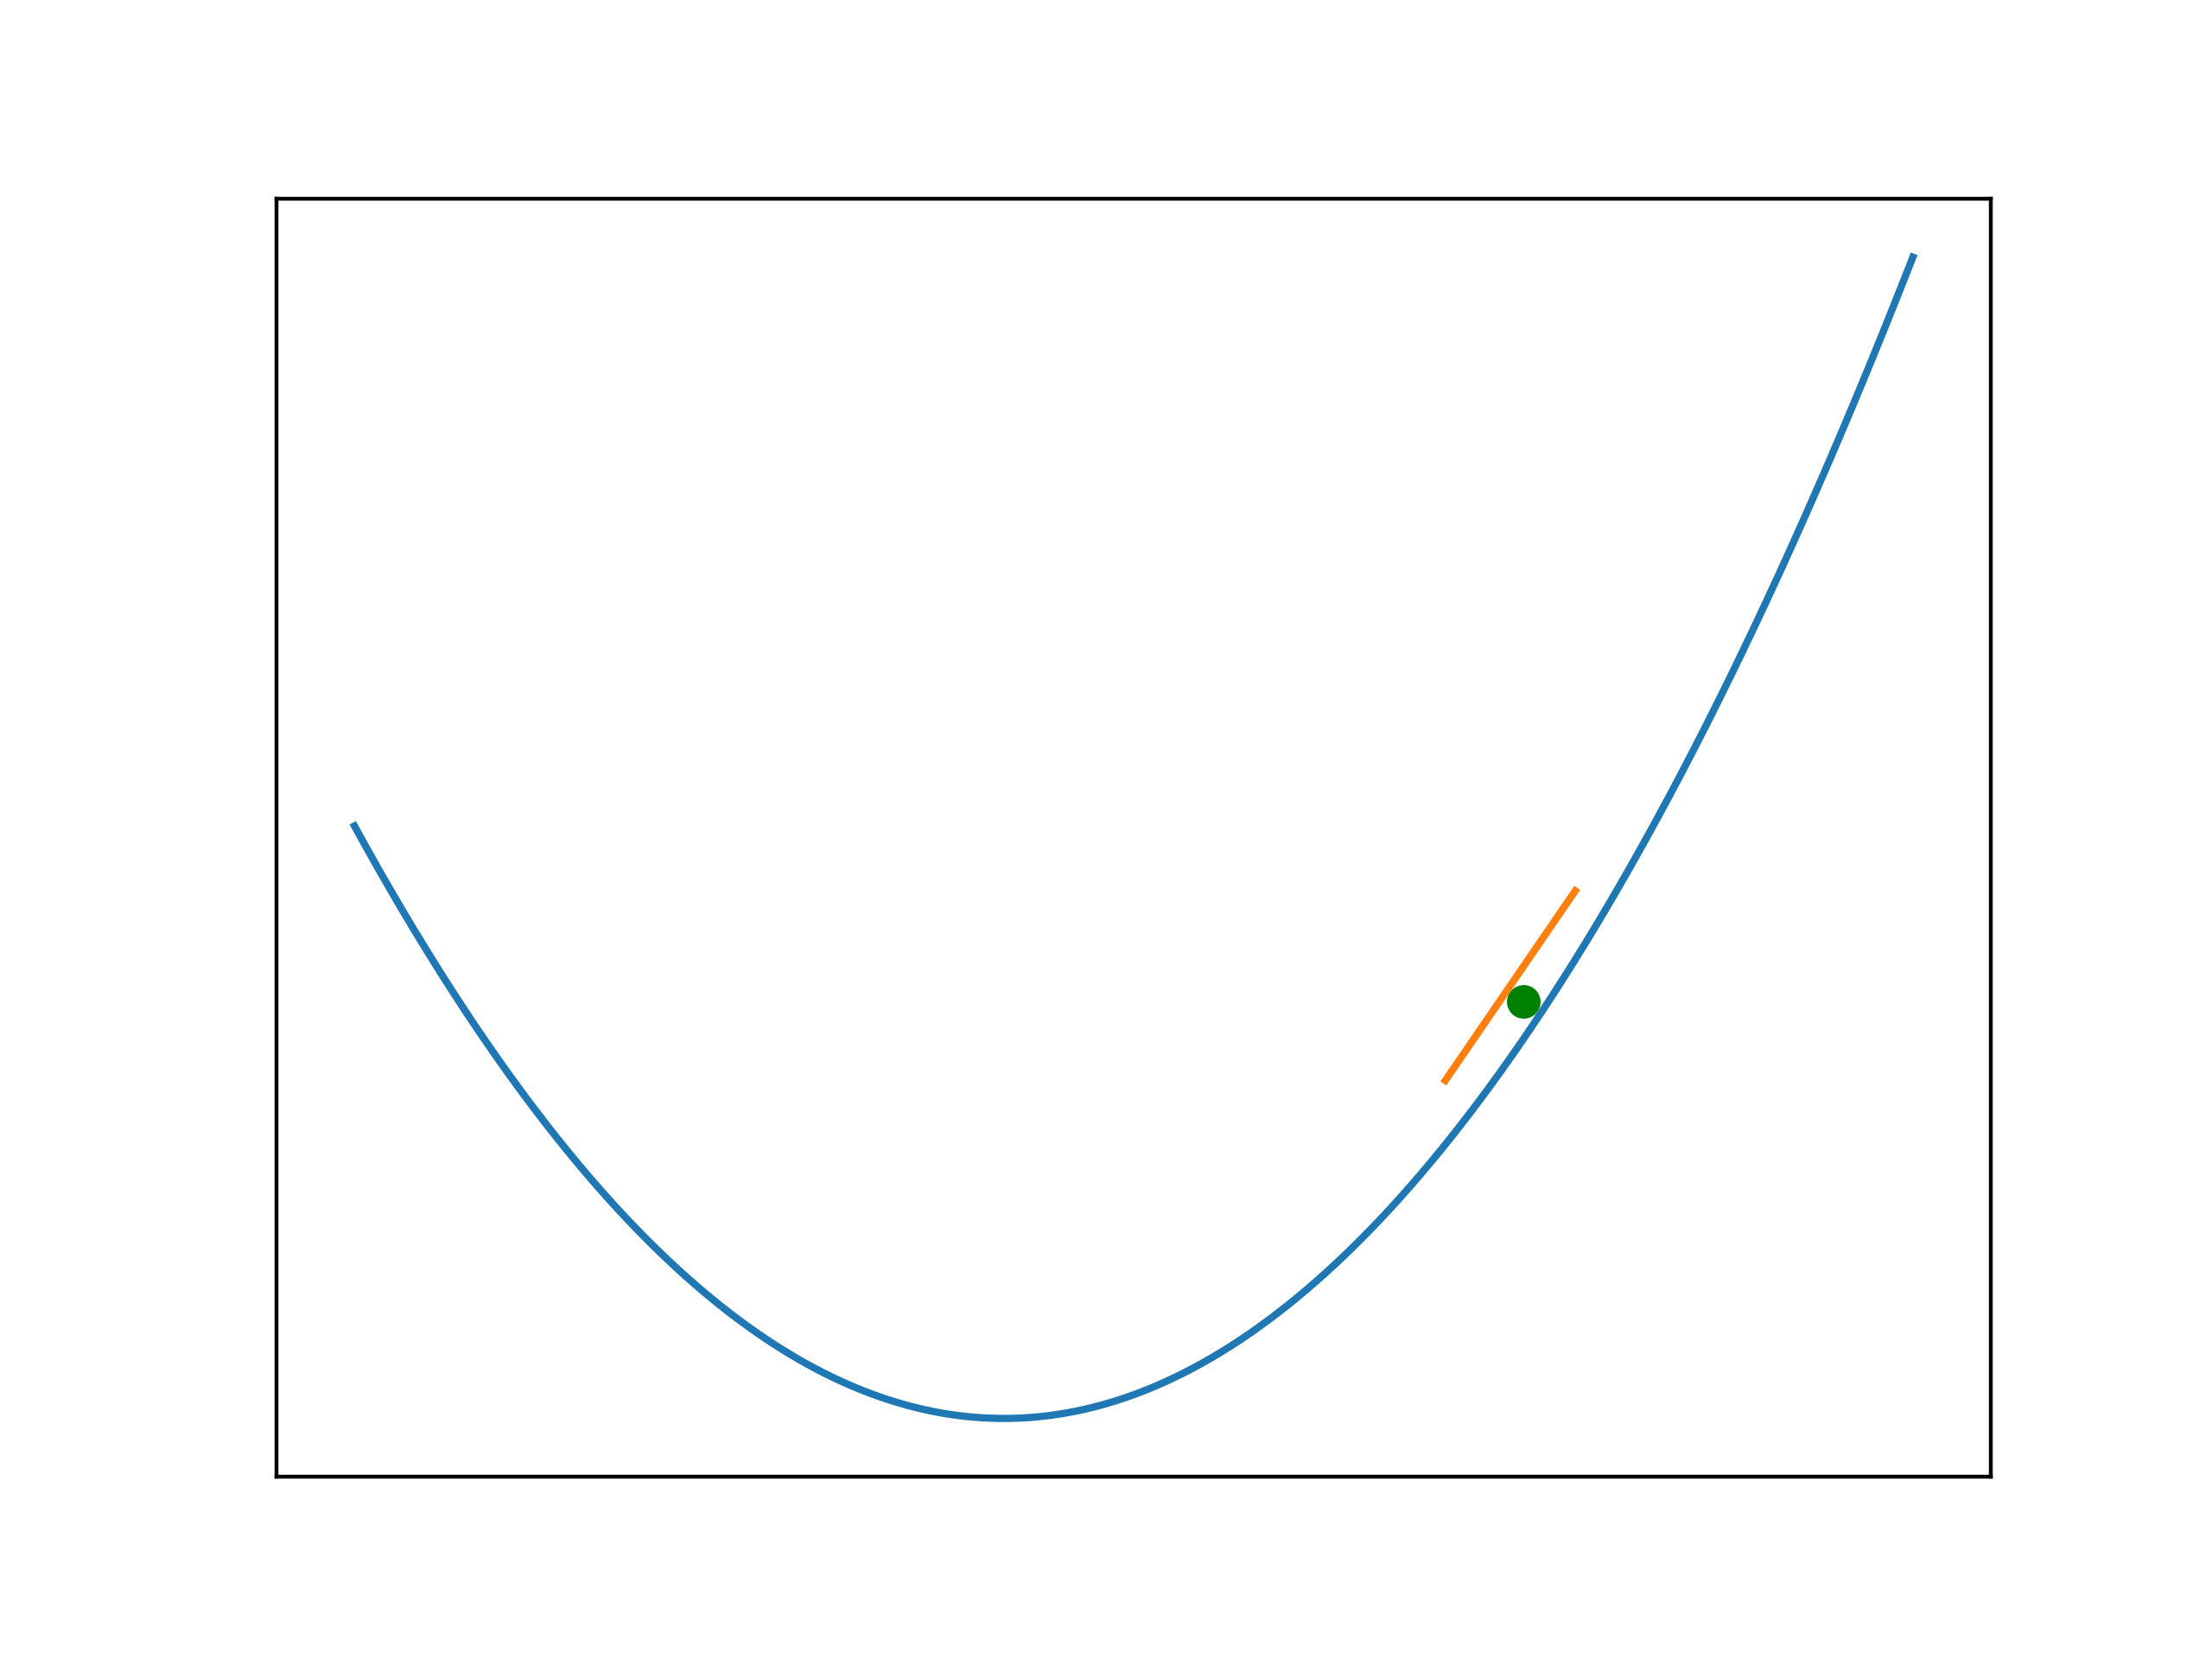
\includegraphics[width=7cm]{figures/background/gradient.png} }}%
    \qquad
    \subfloat[\centering A model parameter's current value as well as it's derivative, headed towards a local minimum.]{{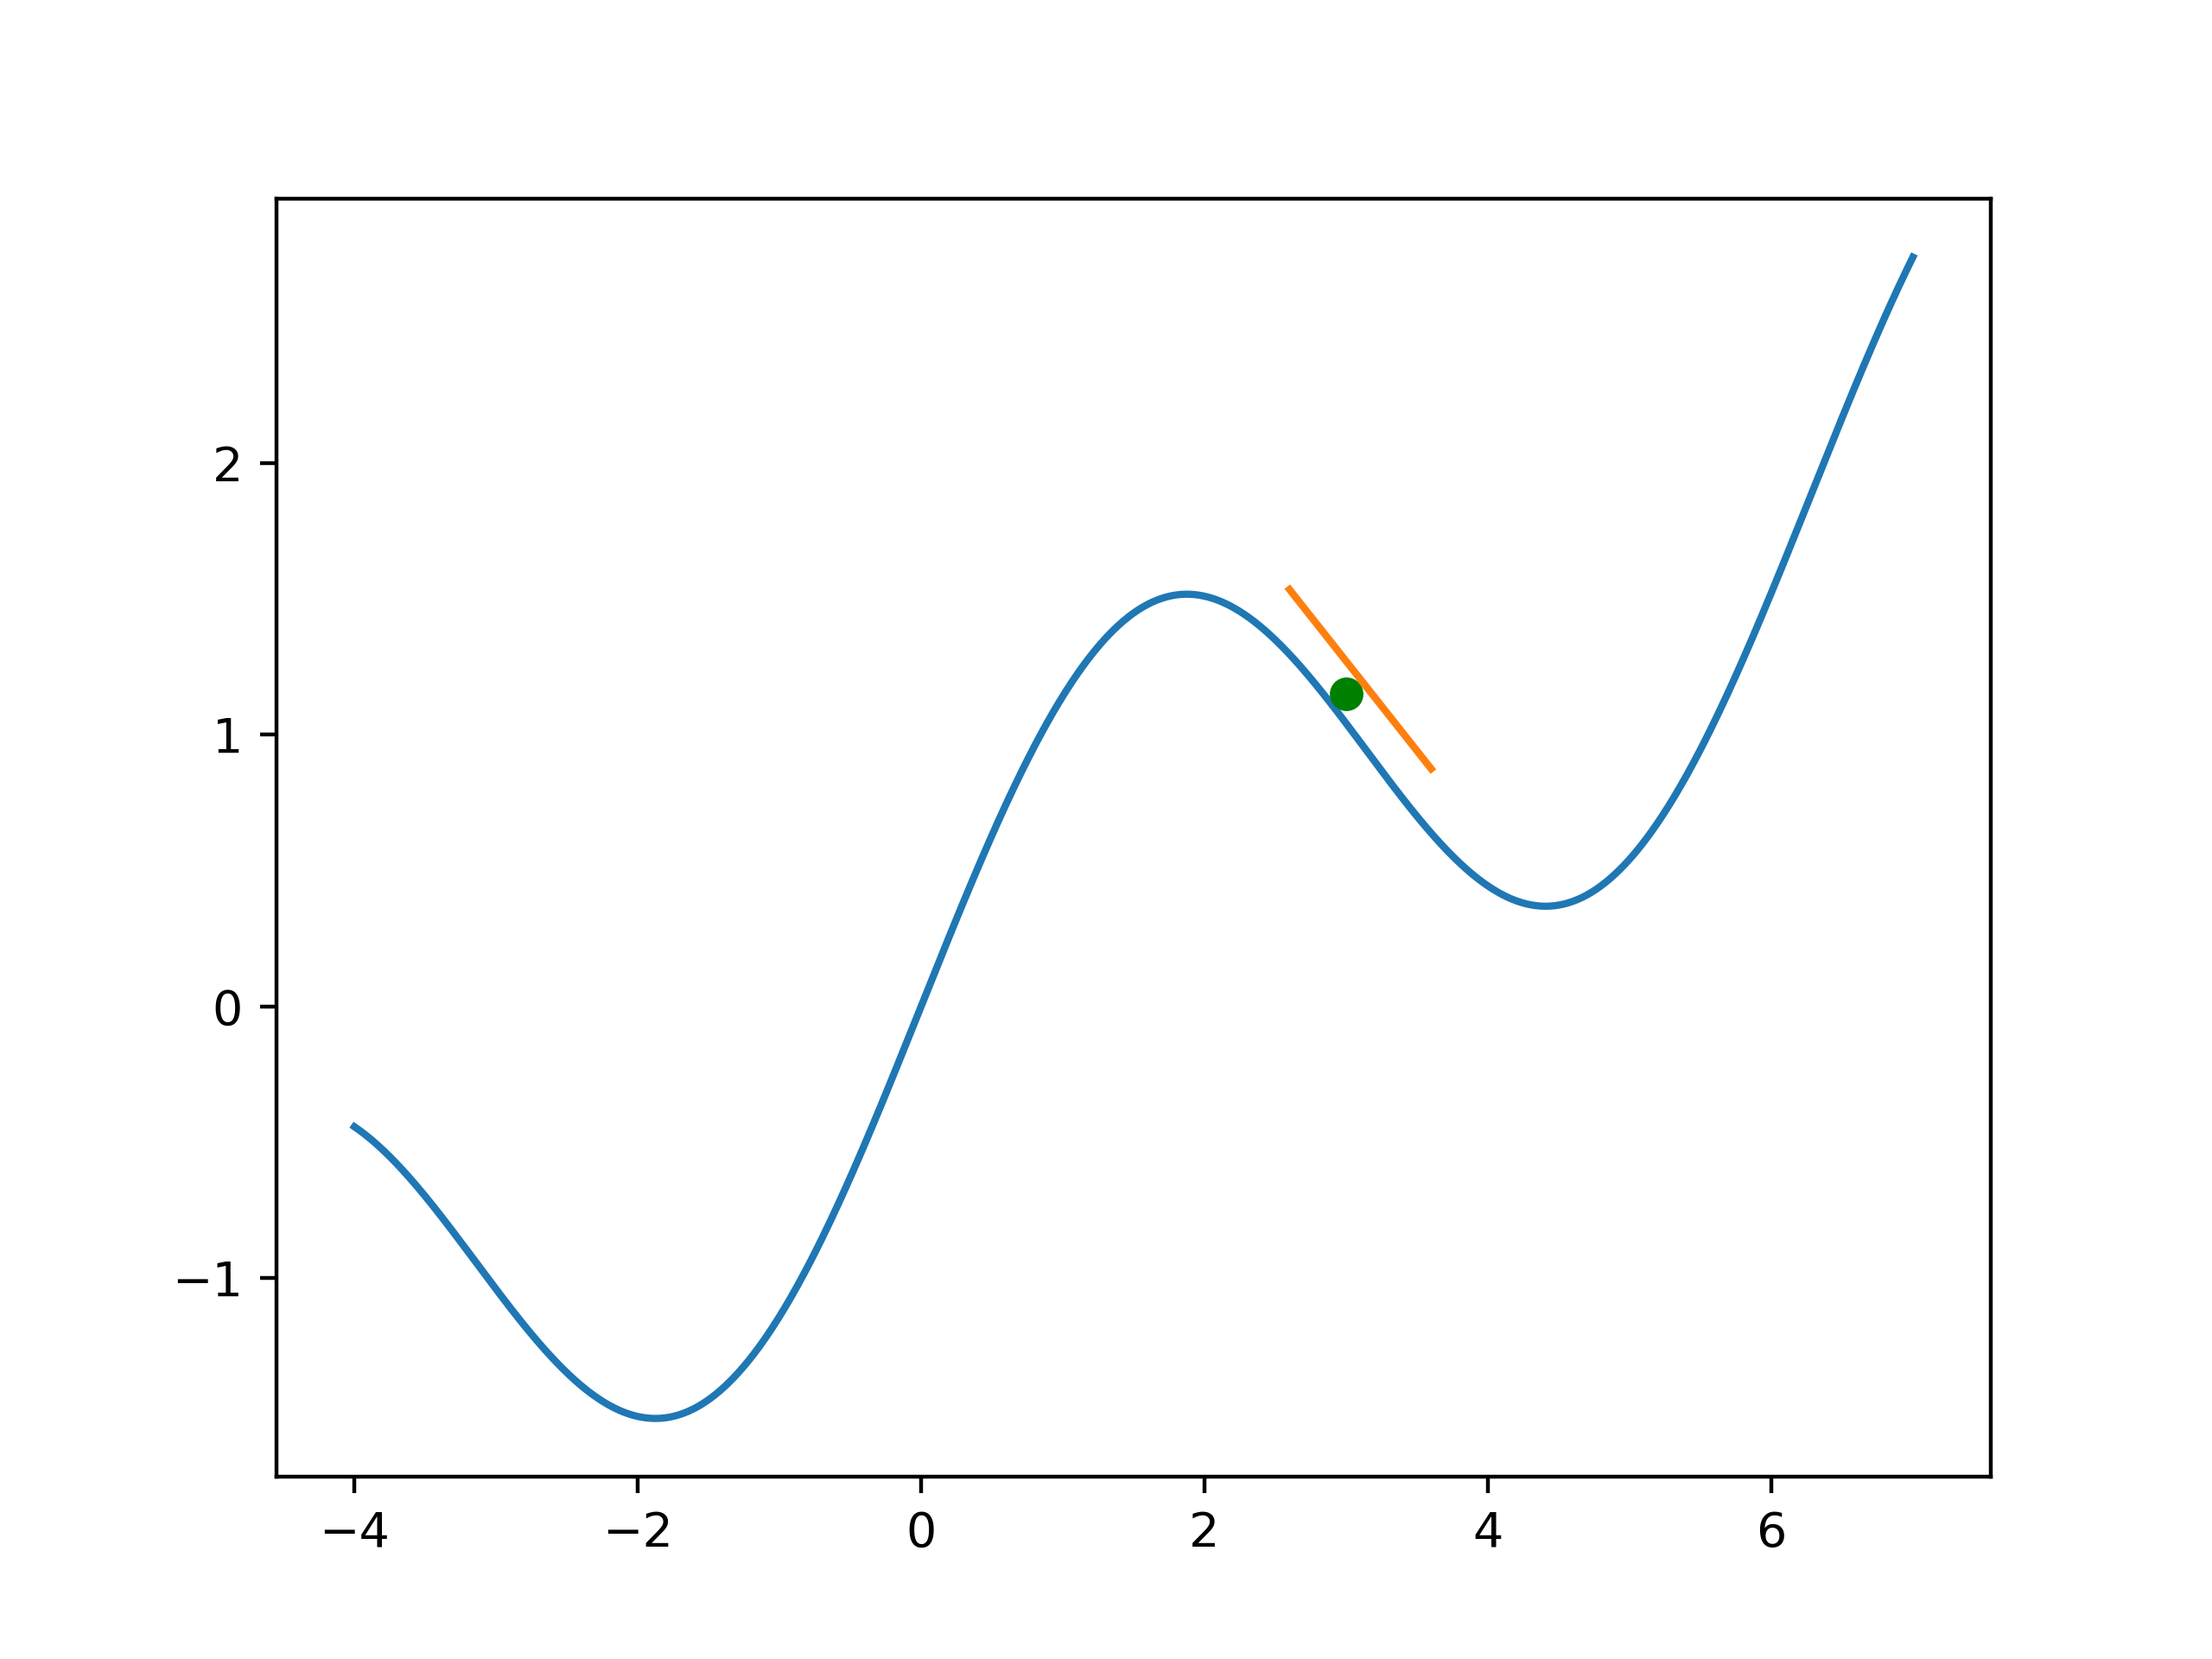
\includegraphics[width=7cm]{figures/background/gradient_local_minimum.png}}}
    \caption{Parameter Gradients}%
    \label{fig:parameter_gradient}%
\end{figure}

The Gradient Descent algorithm utilises the gradient of the model's output in relation to every model parameter
to update each parameter. This idea is illustrated in figure \ref{fig:parameter_gradient}. 
\textcolor{red}{\textbf{Proof?}} It is known that each model parameter has an optimal value that best maps the model's input to desired output.
As there exists a measure of the accuracy of the neural network's prediction and the desired value, 
it is possible to quantify each model parameter's effect on the resulting output. 
This value is given by the derivative of the loss, in relation to the given model parameter.


\textbf{Convergence}

Assume a scenario where at each iteration, a neural network model is trained by providing identical input to the model, 
and it's accuracy is measured by the same target value. Though this method of training the model would provide poor results in any real life application,
it is useful to consider to illustrate the following point. In this scenario, each model parameter's optimal value curve will stay consistent between training iterations.

\textcolor{red}{\textbf{Proof?}} It is obvious then that at each training iteration, 
updating the model parameters in the direction of their respective derivatives' absolute negative values
will result in the model parameters converging either at a local or the global minima,
given that the model is given unlimited training iterations, \textcolor{red}{\textbf{Utdyp her?}} and a decreasing step size.

In such a scenario, the neural network's parameters will converge towards a set of values which optimally maps the model's input to the desired output,
given the initial values of the network's parameters, and the loss function. Figure \ref{fig:parameter_gradient} illustrates that this set of model parameters
may not correspond to the globally optimal set of model parameters. In any case, model parameters trained on identical input data and output data at each iteration
will likely not generalise well to unseen data.

Rather than providing identical input and comparing with identical output at each iteration, new input/output pairs can be provided at every iteration. 
In such a case, the shape of the parameters' derivative loss fuctions as illustrated in figure \ref{fig:parameter_gradient} 
will not remain consistent between training iterations. Instead, the model parameters will converge towards some optimal value
that maps the set of input data to its corresponding output.


\textbf{Chain Rule}

Though calculating the derivative of the loss function in regard to any model parameter may seem like a difficult task, it is in fact elementary.
To calculate the derivative of a given parameter, we utilise the chain rule of derivatives from calculus.
Rodriguez \& Fernández provides the following defintion of the chain rule.

Assume some function $ g(c) $, differentiable at $ c $, and some function $ f(g(c)) $, differentiable at $ g(c) $. 
Then, $ f \circ g $ is differentiable at $ c $, and $ (f \circ g)'(c) = (f' \circ g)(c) \cdot g'(c)  $ \cite{chainRule} 

For the purposes of this thesis, with the same functions and variables as described above, this formulation is rewritten in Leibniz notation, given in formula \ref{func:leibnizChainRule}.

\[
    \frac{\delta f}{\delta c} = \frac{\delta f}{\delta g} \cdot \frac{\delta g}{\delta c} \tag{2.8} \label{func:leibnizChainRule}
\]

In a case where $ g(c) $ can be described by a differentiable equation, a recursive relation is observed, which can be exploited. 
By building neural networks that are differentiable at every part in every layer, calculating the derivative of any parameter in the network then becomes trivial.

To illustrate this property, recall the example network provided in section \ref{subsection:sample_network}. 
In a first scenario, the derivative of network parameter $ w_1^{i,\space j} $ is calculated.

The objective derivative can be stated as $ \frac{\delta \mathcal{L}}{\delta w^{i, j}} $.
Using the formula given in \ref{func:leibnizChainRule}, we redefine this derivative as the product of its chain rule elements.
The derivative is redefined in the following equation.


$$ \frac{\delta \mathcal{L}}{\delta w^{i, \space j}} = \frac{\delta \mathcal{L}}{\delta \hat{y}} \cdot \frac{\hat{y}}{w^{i, \space j}} $$


Assuming MSE loss as defined in \ref{func:mse} is used, and we know the model prediction is a function of the model parameters, 
given a model parameter, we identify the derivative of MSE as the following.


\[
    \frac{\delta MSE^{i, j}}{\delta w_1^{i, \space j}} MSE^{i, j} = 2(y^{i, j} - \hat{y}^{i, j})
\]


No activation function is applied to the output layer in this example instance. Recall then also that $ \hat{y} $ is given as a function $ \hat{y} = W_1 \cdot A_0 + B_1 $. 
It follows that $ \hat{y}(A) $ is differentiable, with the following function.

\[
    \frac{\delta \hat{y}^{i, j}}{\delta w^{i,\space j}} = a_0^{i, \space j}
\]

\textcolor{red}{\textbf{Obs, dette stemmer ikke. Vis til hvordan alle output-verdier påvirker gradient. Vis til at gradient descent itererer over alle train samples før gradient regnes ut.}}


Having calculated the gradient for the given parameter, the parameter is updated in order to minimise the calculated loss in the current iteration. 
The update is limited by some step size, which is a set hyperparameter. The step size may be fixed, or it may decay over time.
The update is described in function \ref{func:gradientUpdate}, in which $ \delta $ is the computed gradient, and $ \gamma $ is the set learning rate.


\[ w^{i, \space j} = w^{i, \space j} - |\delta| \gamma \tag{2.9}  \label{func:gradientUpdate} \]

\textbf{Backpropagation and PyTorch Autograd}

In many pieces of litterature, the term 'optimization step' and the term 'backpropagation'
are used synonymously. While the term 'backpropagation' is often interpreted, it actually
refers to an implementation of the chain rule for calculating model parameter derivatives.
The implementations should utilise dynamic programming to avoid excess computation.
One such implementation is PyTorch's automatic differentiation system named Autograd.

Autograd allows circumventing the computation of the derivatives as they are needed.
Instead, as input data is passed through the model, 
each operation performed using the model parameters are recorded.

A directed acyclic graph in the shape of a tree, with edged pointing towards the root, 
will be generated. 
The current iteration's training input, as well as all model parameters, 
will appear as leaf nodes in the tree.
Mathematical operations performed on the tensors, 
as well as the intermediate states between the operations will be represented as the child nodes of the described leaf nodes.
In each intermediate node, the previous nodes' values will be saved in a context variable.
The calculated loss will be the represented by the tree's root.

This structure allows the PyTorch library to efficiently perform the backward pass.
It needs only to perform the instructions specified at each intermediate node.
Values utilised more than once in the backward pass will only be computed once.
This makes PyTorch's Autograd system an efficient implementation of calculating the gradients,
while still utilising the chain rule. \textbf{\textcolor{red}{dårlig formulert, skriv om.}}





\subsubsection{A note on bayesian statistics}

\subsubsection{Stochastic Gradient Descent}

Though the Gradient Descent algorithm does converge at a set of model parameters, the algorithm is flawed.
The algorithm requires the model to iterate over all samples before computing the gradient and performing the parameter update.
This process is computationally expensive, and may take a long time. 

Rather than iterating over training input, the Stochastic Gradient Descent selects a subset of the training data.
The dataset is shuffled, and at every iteration, a selected number of samples are selected. 
The number of samples used in every iteration is a hyperparameter.
The data is passed through the model, and the loss function is calculated over this quantity.

Subsets of input data are passed through the model, and parameter updates are performed, until all input data has been passed through the model.
This process may then be repeated until the model parameters converge.

By performing the parameter updates in this fashion, far less computation is required for each parameter update.
As a consequence, the neural network's model parameters will converge faster. 
Also, while in the Gradient Descent case, the training target will remain the same every time the parameter gradients are computed.
\textcolor{red}{\textbf{Stemmer dette?}} In the stochastic case, the mean training target will change at each paramter update iteration. 
Training target variation is increased, which also aids the algorithm's convergence property.


\subsubsection{Adam}

Adam is one of many successors of the SGD algorithm. 
It is a notable algorithm, as it has become an industry standard in AI research.
...









\subsection{A sample training loop}
...












% -------------------------------------------------------
% -------------------------------------------------------
% --------------------- Autoencoder ---------------------
% -------------------------------------------------------
% -------------------------------------------------------
\section{Autoencoders}

This section aims to explain the popular neural network architecture referred to as the 'Autoencoder'.


What is today commonly referred to as the 'Autoencoder' was by Kramer in 1989
introduced as 'Nonlinear Principal Components Analysis using Autoassociative Neural Networks'\cite{autoencoderOrigin}.







% -------------------------------------------------------
% -------------------------------------------------------
% ---------------- Graph Neural Networks ----------------
% -------------------------------------------------------
% -------------------------------------------------------
\section{Graph Neural Networks}

The topic of learning on Graphs is well discussed in Bronstein et al.'s Geometric Deep Learning Blueprint \cite{geometricDeepLearningBlueprint}



\subsection{The Convolution Layer}
\subsection{Permutation invariance and equivariance}
\subsection{Attention and Message Passing}
\subsection{Graph Neural Network Architectures}

